\documentclass[a4paper, 11pt]{article}
\usepackage[french]{babel}
\usepackage[utf8]{inputenc} 
\usepackage[T1]{fontenc}
\usepackage{multirow, multicol}
\usepackage{amsmath, amssymb, latexsym}
\usepackage{graphicx, epsfig,subfigure}
\usepackage[lined,boxed]{algorithm}
\usepackage{algorithmic}
\usepackage{rotate}
\usepackage{url}
\usepackage{setspace}
\usepackage{fancyhdr}
\usepackage{color}
\usepackage{hyperref} 

\newtheorem{definition}{Definition}
\newtheorem{example}{Example}
\newtheorem{proposition}{Proposition}
\newtheorem{proof}{Proof}
\pagestyle{fancy}
\fancyhf{}
\newcommand{\univ}{
\epsfig{file = images/logoUni.png, height = 1.05cm}}
\lhead{\univ}
\rhead{\date{\today}}
\rfoot{Page \thepage}

\title{}
\author{CHAMPENOIS Brandon \textsc{G5B} \\ BONVARLET Bastien \textsc{G5B} \\ MASSON Joris \textsc{G5B} }

\begin{document}
\maketitle
\centerline{
\includegraphics[width = 7cm]{images/ecos.png}}
\tableofcontents
\newpage

\section{Rapide présentation / résumé du projet}
Notre projet est une simulation d'écosystème\\

\subsection*{Qu'est-ce qu'une simulation d'écosystème ?}
Tout d'abord qu'est-ce qu'une simulation d'écosystème ?\\
Alors une simulation d'écosystème c'est une simulation de vie, reprenant plusieurs critères comme :\\
La reproduction, chasse, "guerre", faim...\\

\subsection{Ce que fait notre simulation}
Nos avons décider de donner la nom Ecos a notre projet, car nous n'avions pas trouver d'autre idées que de raccourcir le mots écosystème en Ecos. Notre simulation contient 5 espèces différentes : l'humain, l'orc, l'ours, le loup, le lapin. Nous avons donc ajouter des "armes": un caillou et un bâton. Pour ce qui est de la nourritures nos entités étant majoritairement carnivores, nous n'avons pas eu besoin de rajouter beaucoup de choses pour la nourriture si ce n'est de l'herbe pour le lapin qui est tout en bas de la chaîne alimentaire de notre simulation.\\
\subsection{Architecture du projet}
\subsubsection{Explication de l'architecture du projet:}
Notre projet est organisé de manière à ce que chaque programme, dossier et autres fichiers puisses communiquer ensemble assez facilement.\\
Nous avons un dossier intitulé "ecos\_pour\_python\_machine\_fac", il est indépendant de ecos puisqu'il reprend tout le projet pour pyton 3.8.\\
\newpage

\subsubsection{arborescence du projet :}
\begin{figure*}[ht!]
 \centering
 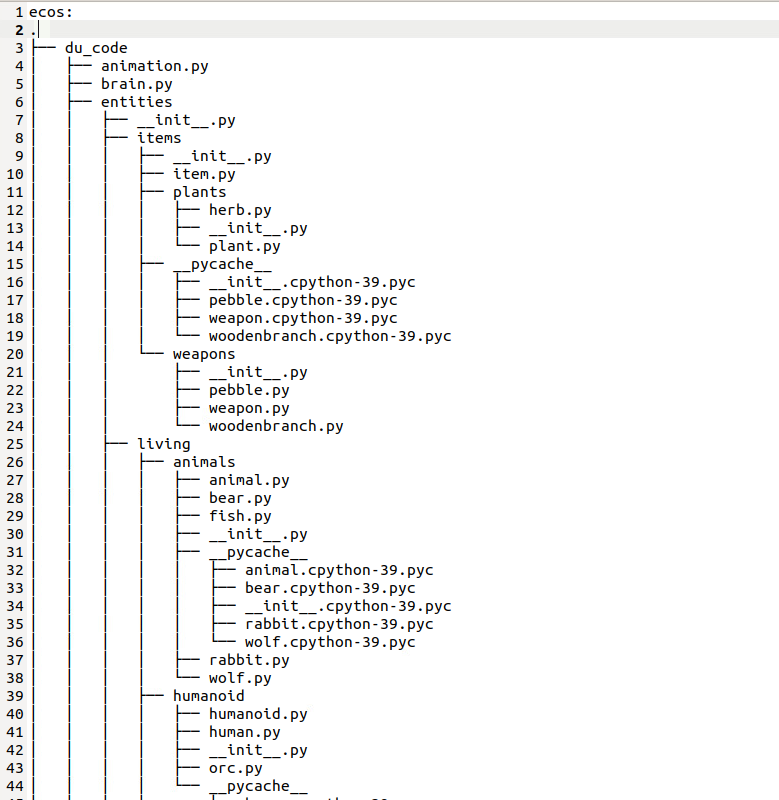
\includegraphics[width=0.5\linewidth]{images/arborecsens/arbrepart1.png}
 \caption{partie 1 de l'arborescence}
 \label{fig::example::one}
\end{figure*}
\begin{figure*}[ht!]
 \centering
 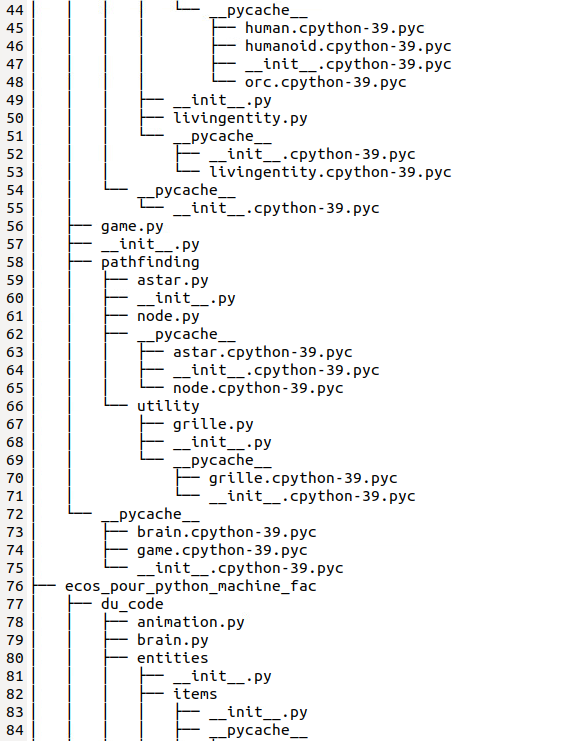
\includegraphics[width=0.5\linewidth]{images/arborecsens/arbrepart2.png}
 \caption{partie 2 de l'arborescence}
 \label{fig::example::one}
\end{figure*}
\begin{figure*}[ht!]
 \centering
 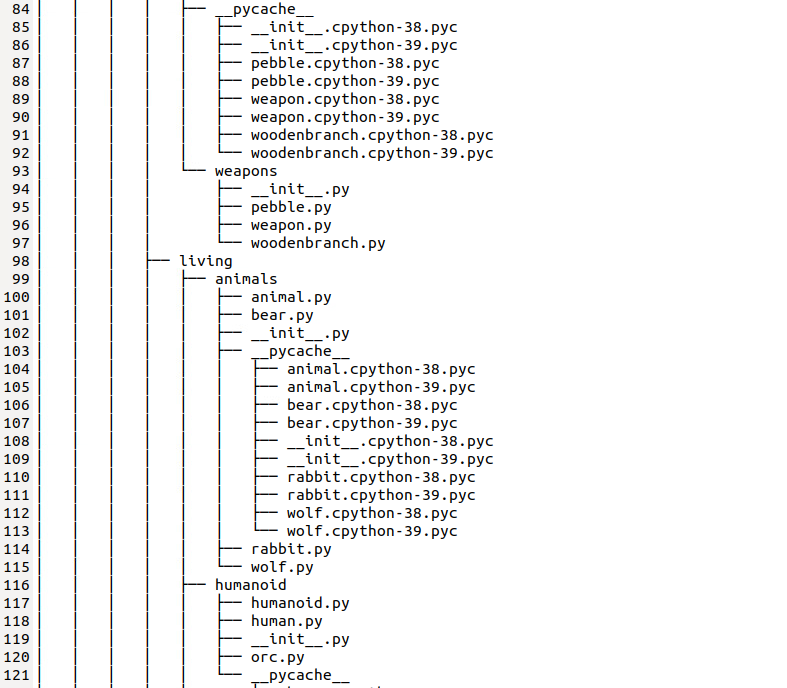
\includegraphics[width=0.5\linewidth]{images/arborecsens/arbrepart3.png}
 \caption{partie 3 de l'arborescence}
 \label{fig::example::one}
\end{figure*}
\begin{figure*}[ht!]
 \centering
 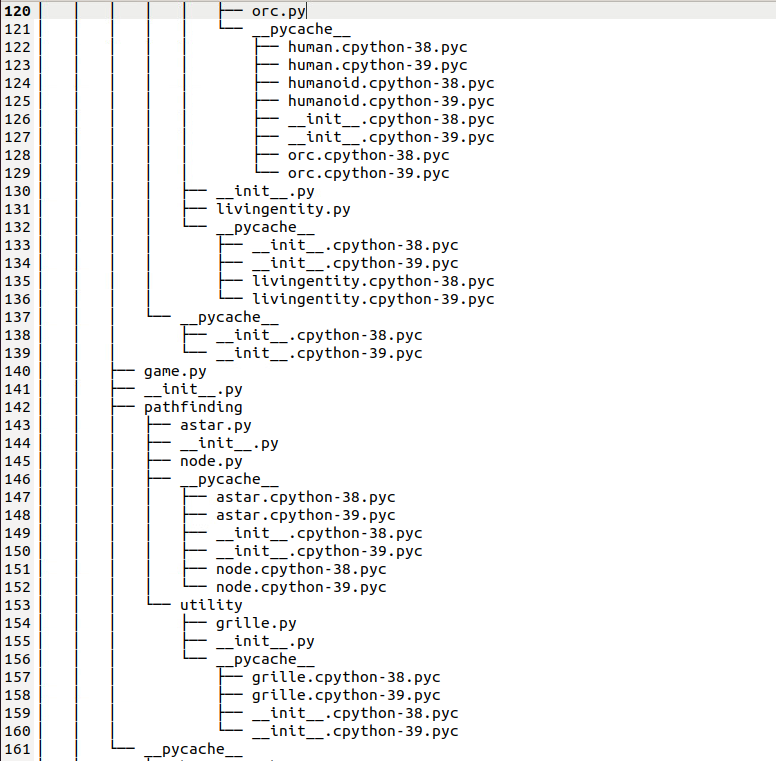
\includegraphics[width=0.5\linewidth]{images/arborecsens/arbrepart4.png}
 \caption{partie 4 de l'arborescence}
 \label{fig::example::one}
\end{figure*}
\newpage
{\color{white}Ceci sert a la mise en page}
\newpage
\begin{figure*}[ht!]
 \centering
 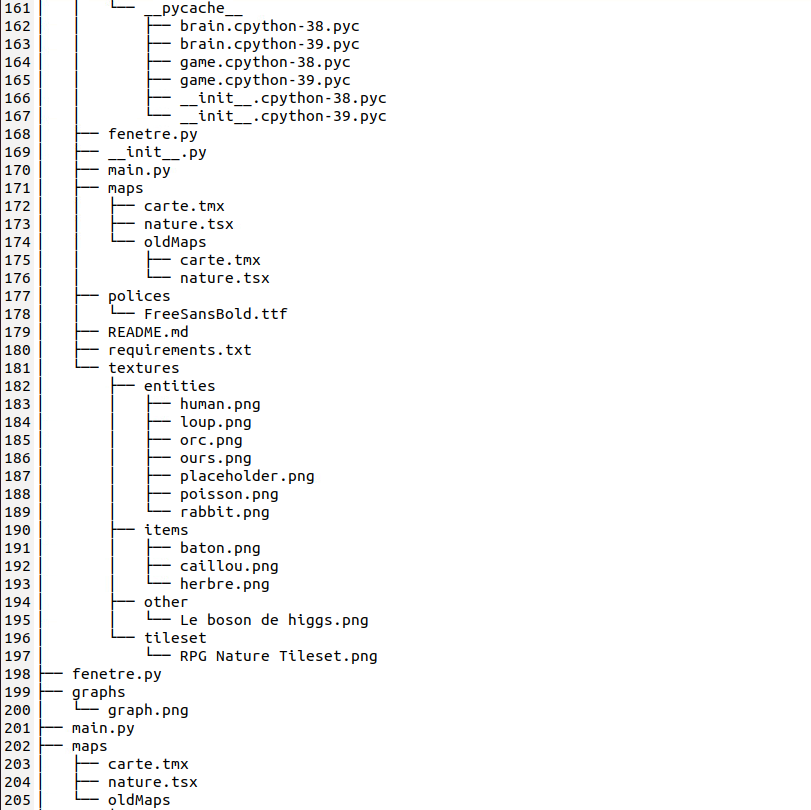
\includegraphics[width=0.5\linewidth]{images/arborecsens/arbrepart5.png}
 \caption{partie 5 de l'arborescence}
 \label{fig::example::one}
\end{figure*}
\begin{figure*}[ht!]
 \centering
 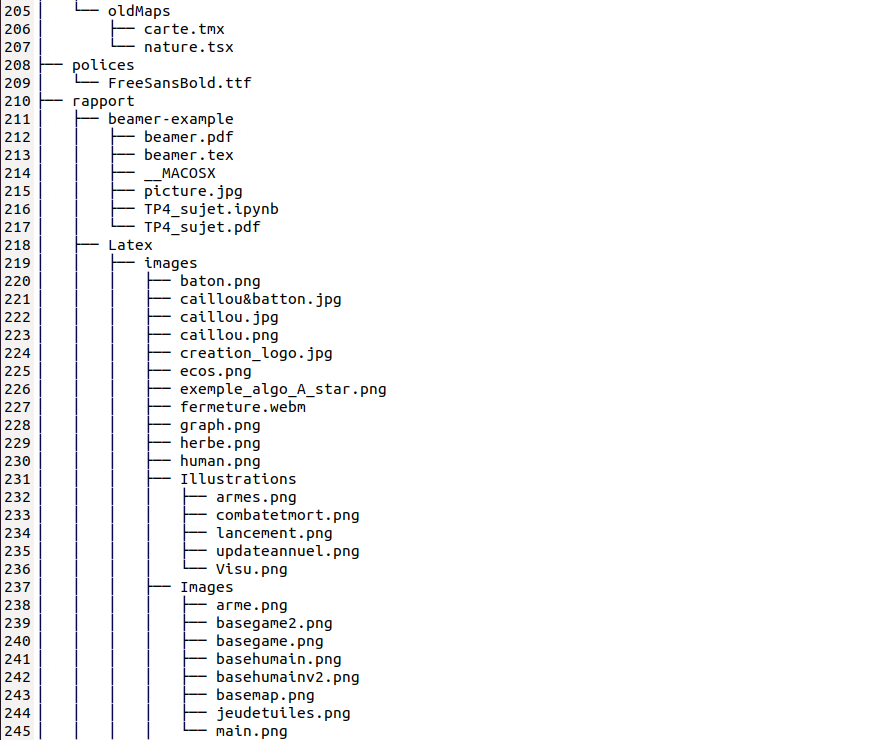
\includegraphics[width=0.5\linewidth]{images/arborecsens/arbrepart6.png}
 \caption{partie 6 de l'arborescence}
 \label{fig::example::one}
\end{figure*}
\newpage
{\color{white}Ceci sert a la mise en page}

\begin{figure*}[ht!]
 \centering
 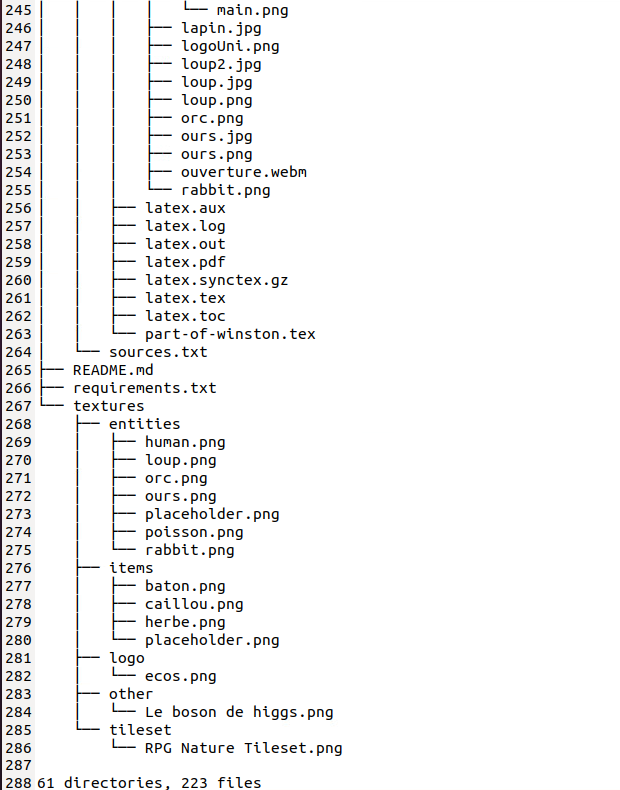
\includegraphics[width=0.5\linewidth]{images/arborecsens/arbrepart7.png}
 \caption{partie 7 de l'arborescence}
 \label{fig::example::one}
\end{figure*}
{\color{white}Ceci sert a la mise en page}
\newpage

\section{Manuel d'utilisation de l'application }

Tout d'abord pour lancer l'application, il suffit d’exécuter le main.py. Qui lui même exécutera le fichier fenetre.py qui exécutera une fenêtre de 500 * 700 pixels de là nous aurons deux possibilités soit arrêter l'application via le bouton "Quitter", soit exécuter le fichier game.py via le bouton "lancer". Si vous appuyer sur "quitter" la fenêtre se fermera. Si vous appuyer sur "lancer" qui exécutera à son tour le fichier game.py. Le fichier game.py génère une fenêtre de jeu de 1050 * 800 pixels qui va générer la carte sur 800 * 800 pixels où les entités apparaîtrons de manière aléatoire sur la carte
sur la droite de la fenêtre nous aurons des informations tel que les jours, années écoulées et le nombre d'entité par espèces en temps réel et un graphique sur l'évolution de la population de chaque espèces.\\
Nos entités vivantes se déplacent selon un tuple aléatoire et on leur demande d'aller jusque la avec l'algorithme, cela dépend également des conditions de faim.\\
Notre algorithme est basé sur l'algorithme A* ou A star ou encore A étoile. Cet algorithme va regarder les cases alentours, puis leur calculer un score, la case ayant le score le plus bas va l'emporter et l'algorithme va donc prendre cette case pour référence et l'algorithme va recommencer jusqu'à arriver a destination. Le calcul du score se fait en additionnant deux valeurs: la distance de Manhattan jusqu'à la destination et une autre distance de Manhattan entre la destination et la case parente à celle dont on calcule le score.\\
\\
Le principe de cet algorithme et de trouver et de suivre le chemin le plus rapide pour arriver a destination, et ce, le plus rapidement possible, le chemin trouvé ne sera peut-être pas le plus rapide, mais il sera trouvé rapidement, ce qui est parfait lorsque l'on doit l'exécuter énormément.
\begin{figure*}[ht!]
 \centering
 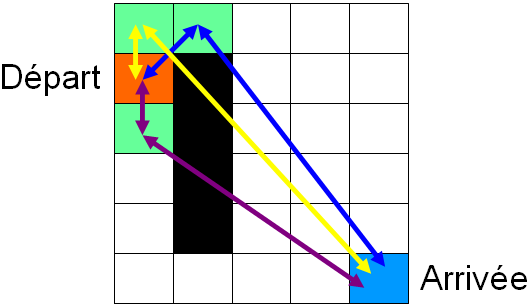
\includegraphics[width=\linewidth]{images/exemple_algo_A_star.png}
 \caption{exemple de l'algorithme A* (A star)}
 \label{fig::example::one}
\end{figure*}
\newpage

\section{Qui a fait quoi ?}

\begin{itemize}
\item Bonvarlet bastien : la base des classes, la base du jeu et base graphique, la map, tentative de gestion des animations.\\
\item Masson Joris : l'algorithme, le game.py, la reproduction, les combats\\
\item Champenois Brandon : Le menu du jeu, le rapport latex, les sprites de chaque entités
\end{itemize}

\subsection{Résumé de ce qui a était fait durant les semaines du projet}

Bonvarlet Bastien :\\
\begin{enumerate}
\item Pour toutes les modifs pour la map et les bases graphiques et codes du log : A passer une dizaine d'heures sur les deux premières semaines.\\
\item Pour la gestion des déplacements de base : a peu près 1-2 heures en tout.\\
\item Pour la création du logo : a peu près 1-2 heures en tout.\\
\item Pour la tentative d'animations : a peu près 2-3 heures en tout. Pour les animations le problème venait du fait que les sprites n'ont pas tous le même nombre d'images et qu'il aurai fallu séparer les sprites en images ou séparer les sprites en sélectionnant les images une par une et en les ajoutant à des listes de déplacements par entité afin de faire défiler les animations (liste pour aller en avant, une autre pour aller en arrière)...\\
\begin{figure*}[ht!]
 \centering
 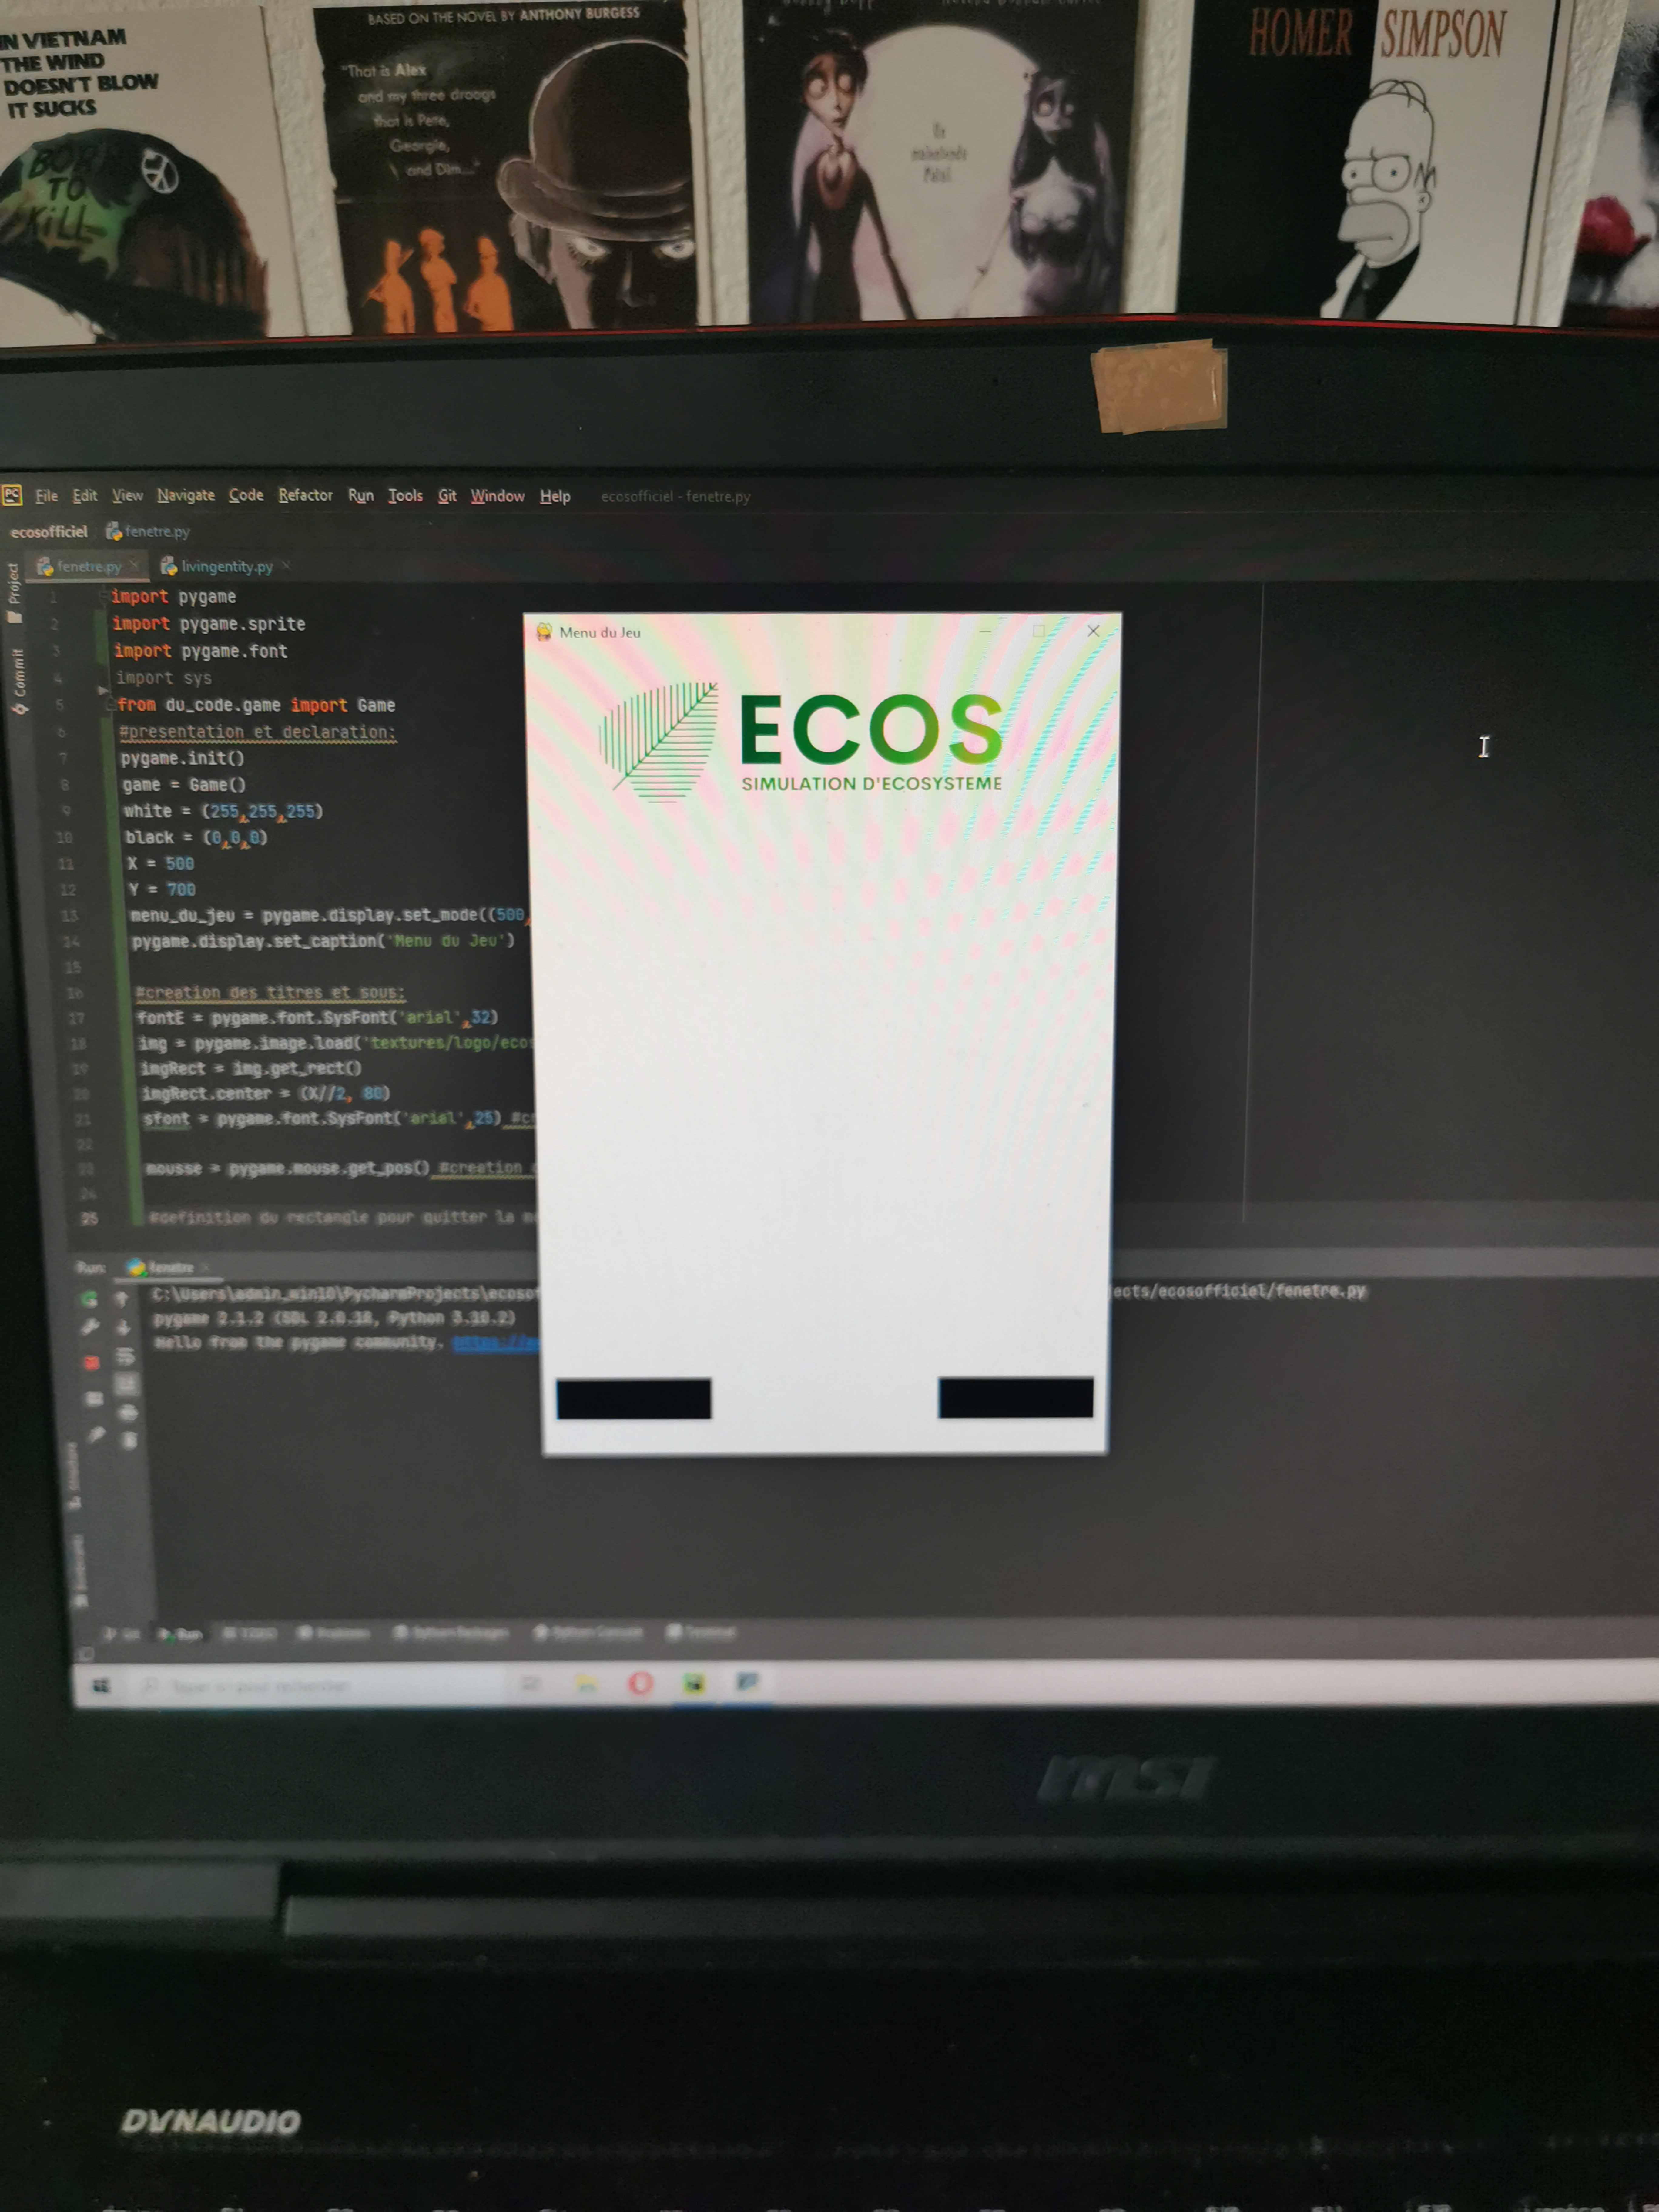
\includegraphics[width=0.5\linewidth]{images/creation_logo.jpg}
 \caption{logo final}
 \label{fig::example::one}
\end{figure*}
\item Pour les animations : \\
\item Pour le sprite du lapin :\\
\begin{figure*}[ht!]
 \centering
 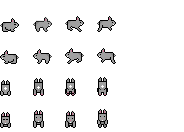
\includegraphics[width=0.75\linewidth]{images/rabbit.png}
 \caption{sprite du lapin}
 \label{fig::example::one}
\end{figure*}
Cela lui a pris environ 4 heures.
\end{enumerate}
\newpage
Masson Joris : \\
\begin{enumerate}
\item Il a passé environ 15-20 heures sur l’algorithme  A* réparti sur 2-3 semaines.\\
\item Il a passé environ 6 heures sur la reproduction, les combats et la faim.\\
\item Il a fait un système de graphique avec matplotlib, il y a consacré une dizaines d'heures:\\
\begin{figure*}[ht!]
 \centering
 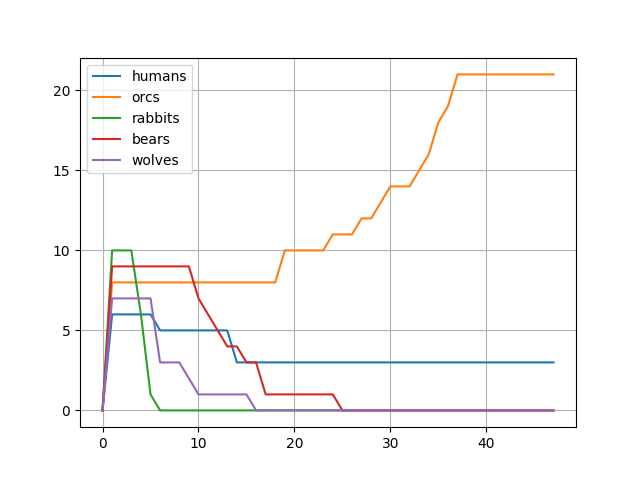
\includegraphics[width=1\linewidth]{images/graph.png}
 \caption{exemple de graphique}
 \label{fig::example::one}
\end{figure*}
\item Il a fait le beamer du 18/04 à maintenant.\\
\end{enumerate}
\newpage
Champenois Brandon : \\
\begin{enumerate}
\item Durant les 3 premières semaines a fait tout les sprites de notre simulation d'écosystème :\\
\item Après avoir récupérer le sprite de l'humain :
\\
\begin{figure*}[ht!]
 \centering
 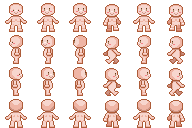
\includegraphics[width=0.5\linewidth]{images/human.png}
 \caption{sprite de l'humain}
 \label{fig::example::one}
\end{figure*} 
\\
\item A fait l'orc il lui suffisait juste de recolorer le sprite de l'humain :
\\ 
\begin{figure*}[ht!]
 \centering
 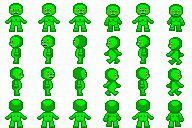
\includegraphics[width=0.5\linewidth]{images/orc.png}
 \caption{sprite de l'orc}
 \label{fig::example::one}
\end{figure*}
\\
Cela lui a pris 3-4 heures\\
\\
\item Il a donc ensuite fait des croquis pour les autres entités :
\\
\begin{figure*}[ht!]
  \begin{minipage}[c]{.5\linewidth}
   \centering
   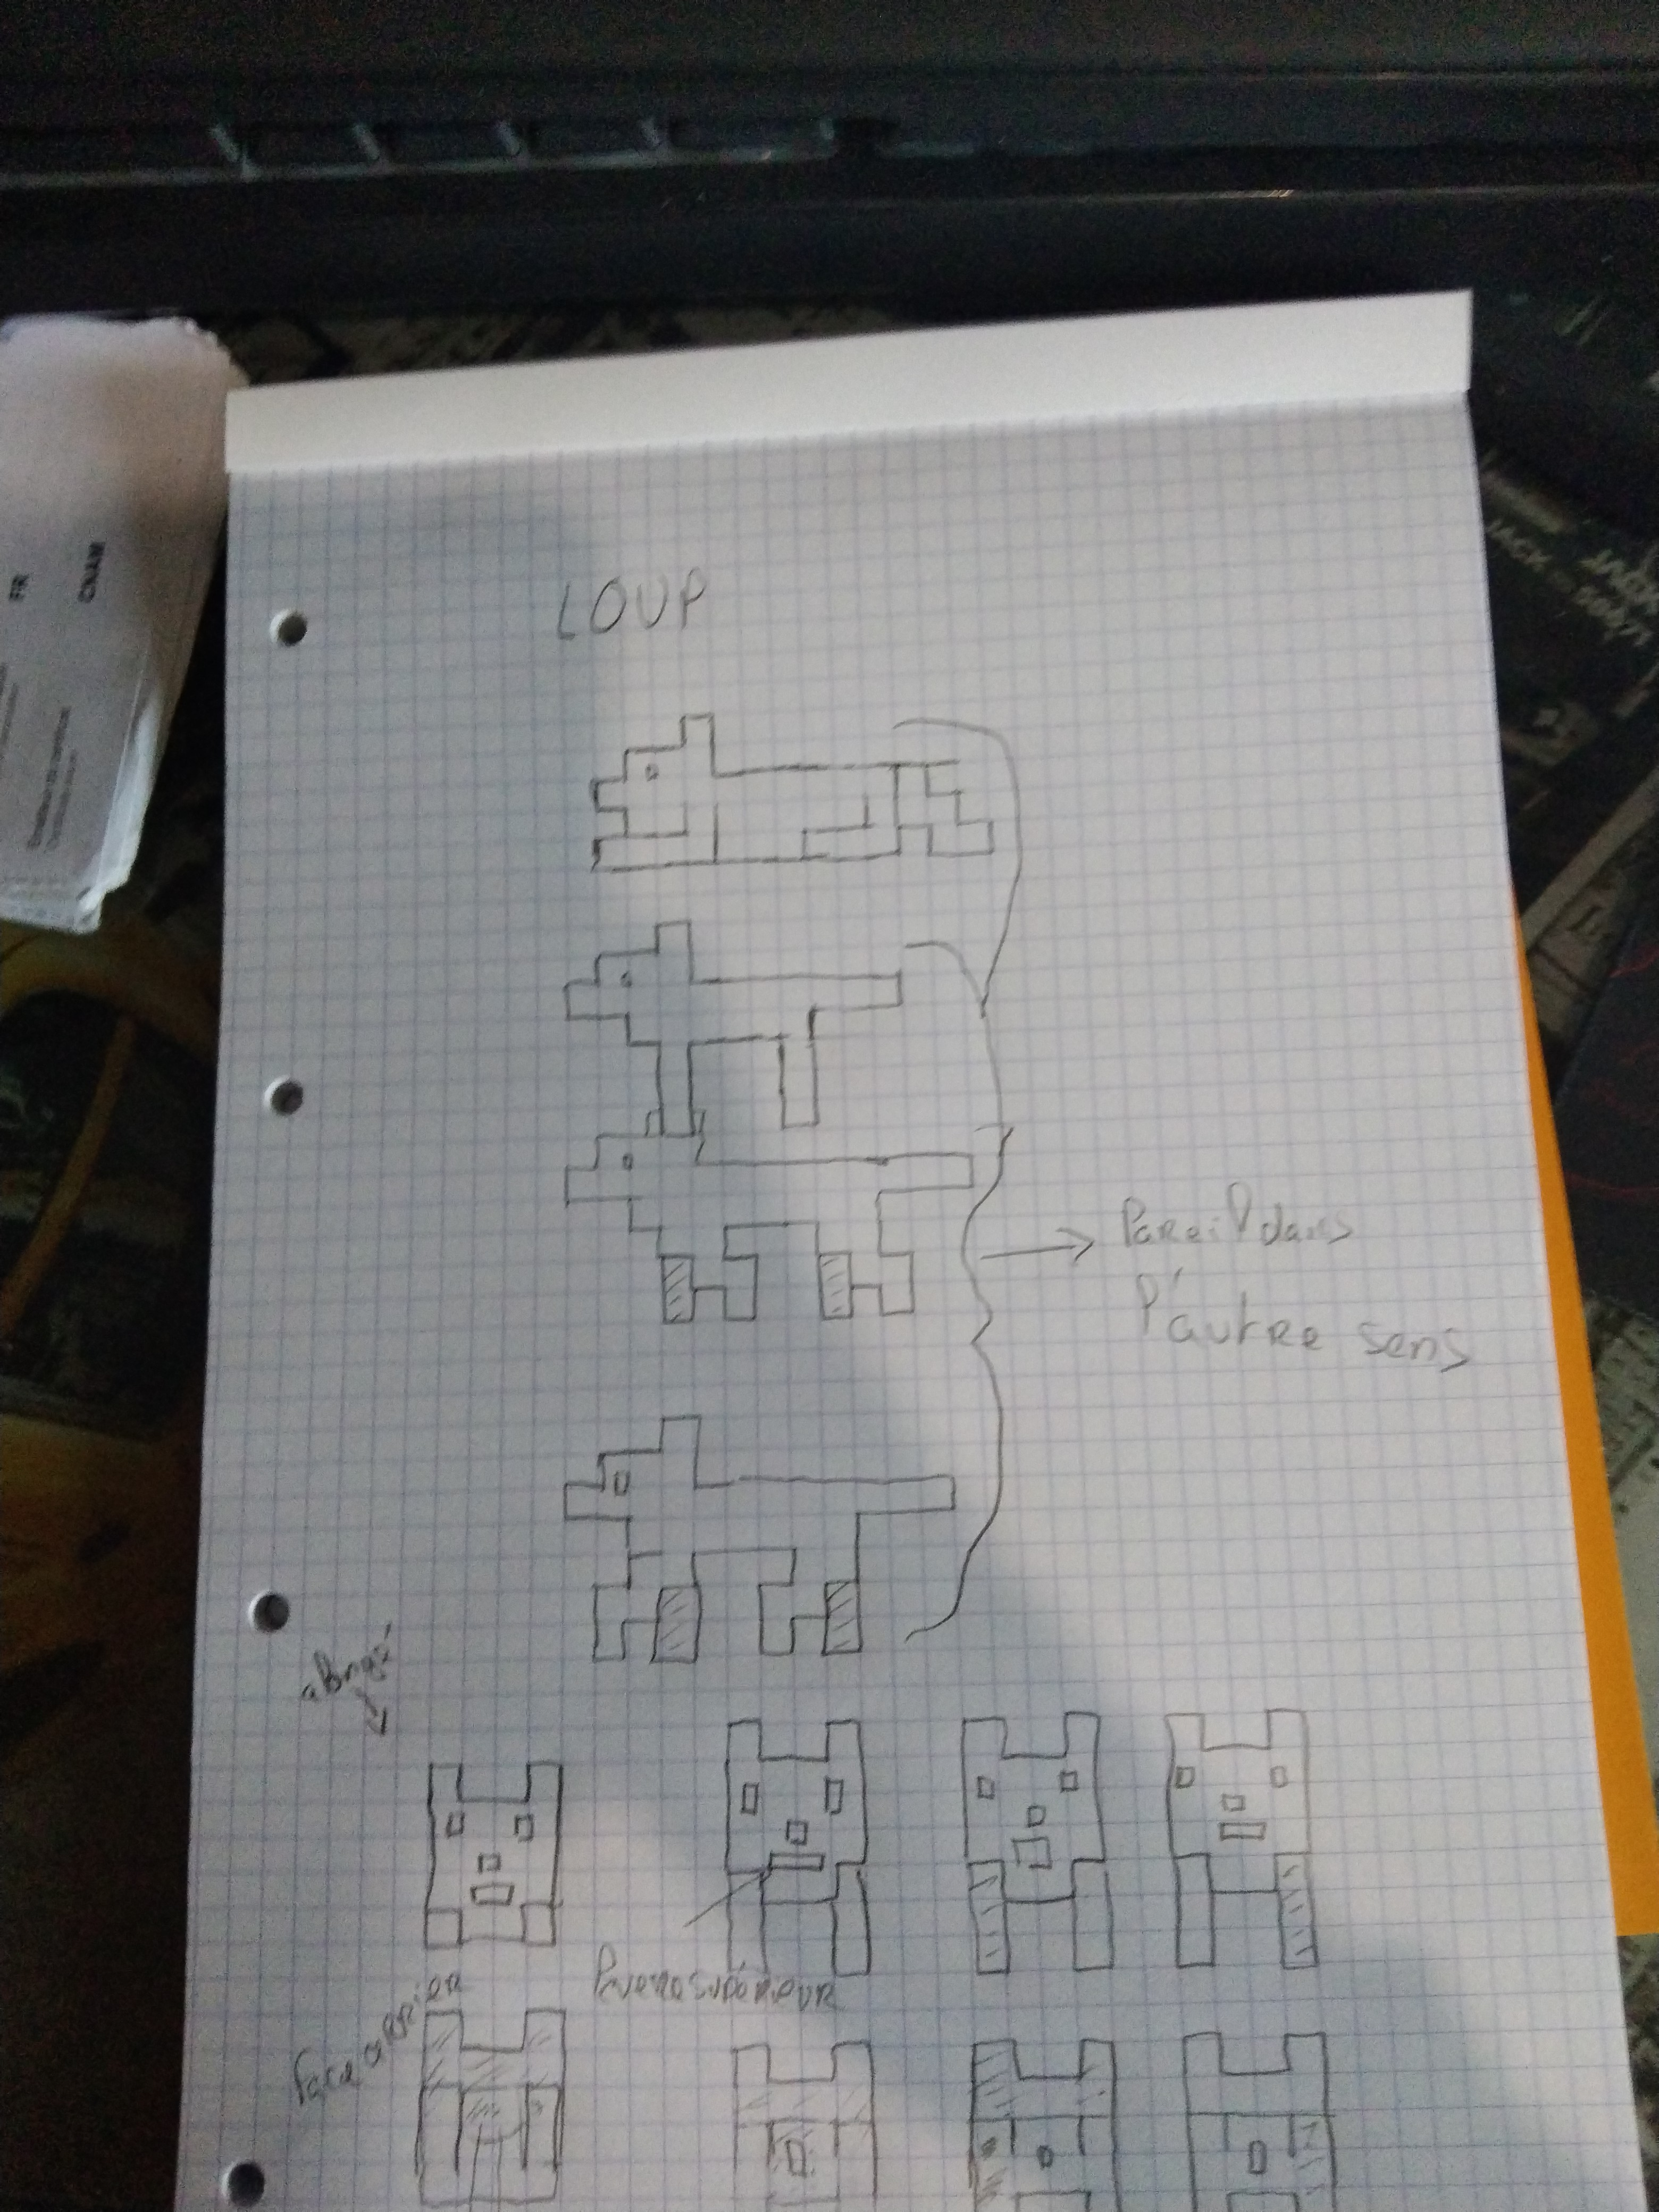
\includegraphics[width=\linewidth]{images/loup.jpg}
  \end{minipage} \hfill
  \begin{minipage}[c]{.5\linewidth}
   \centering
   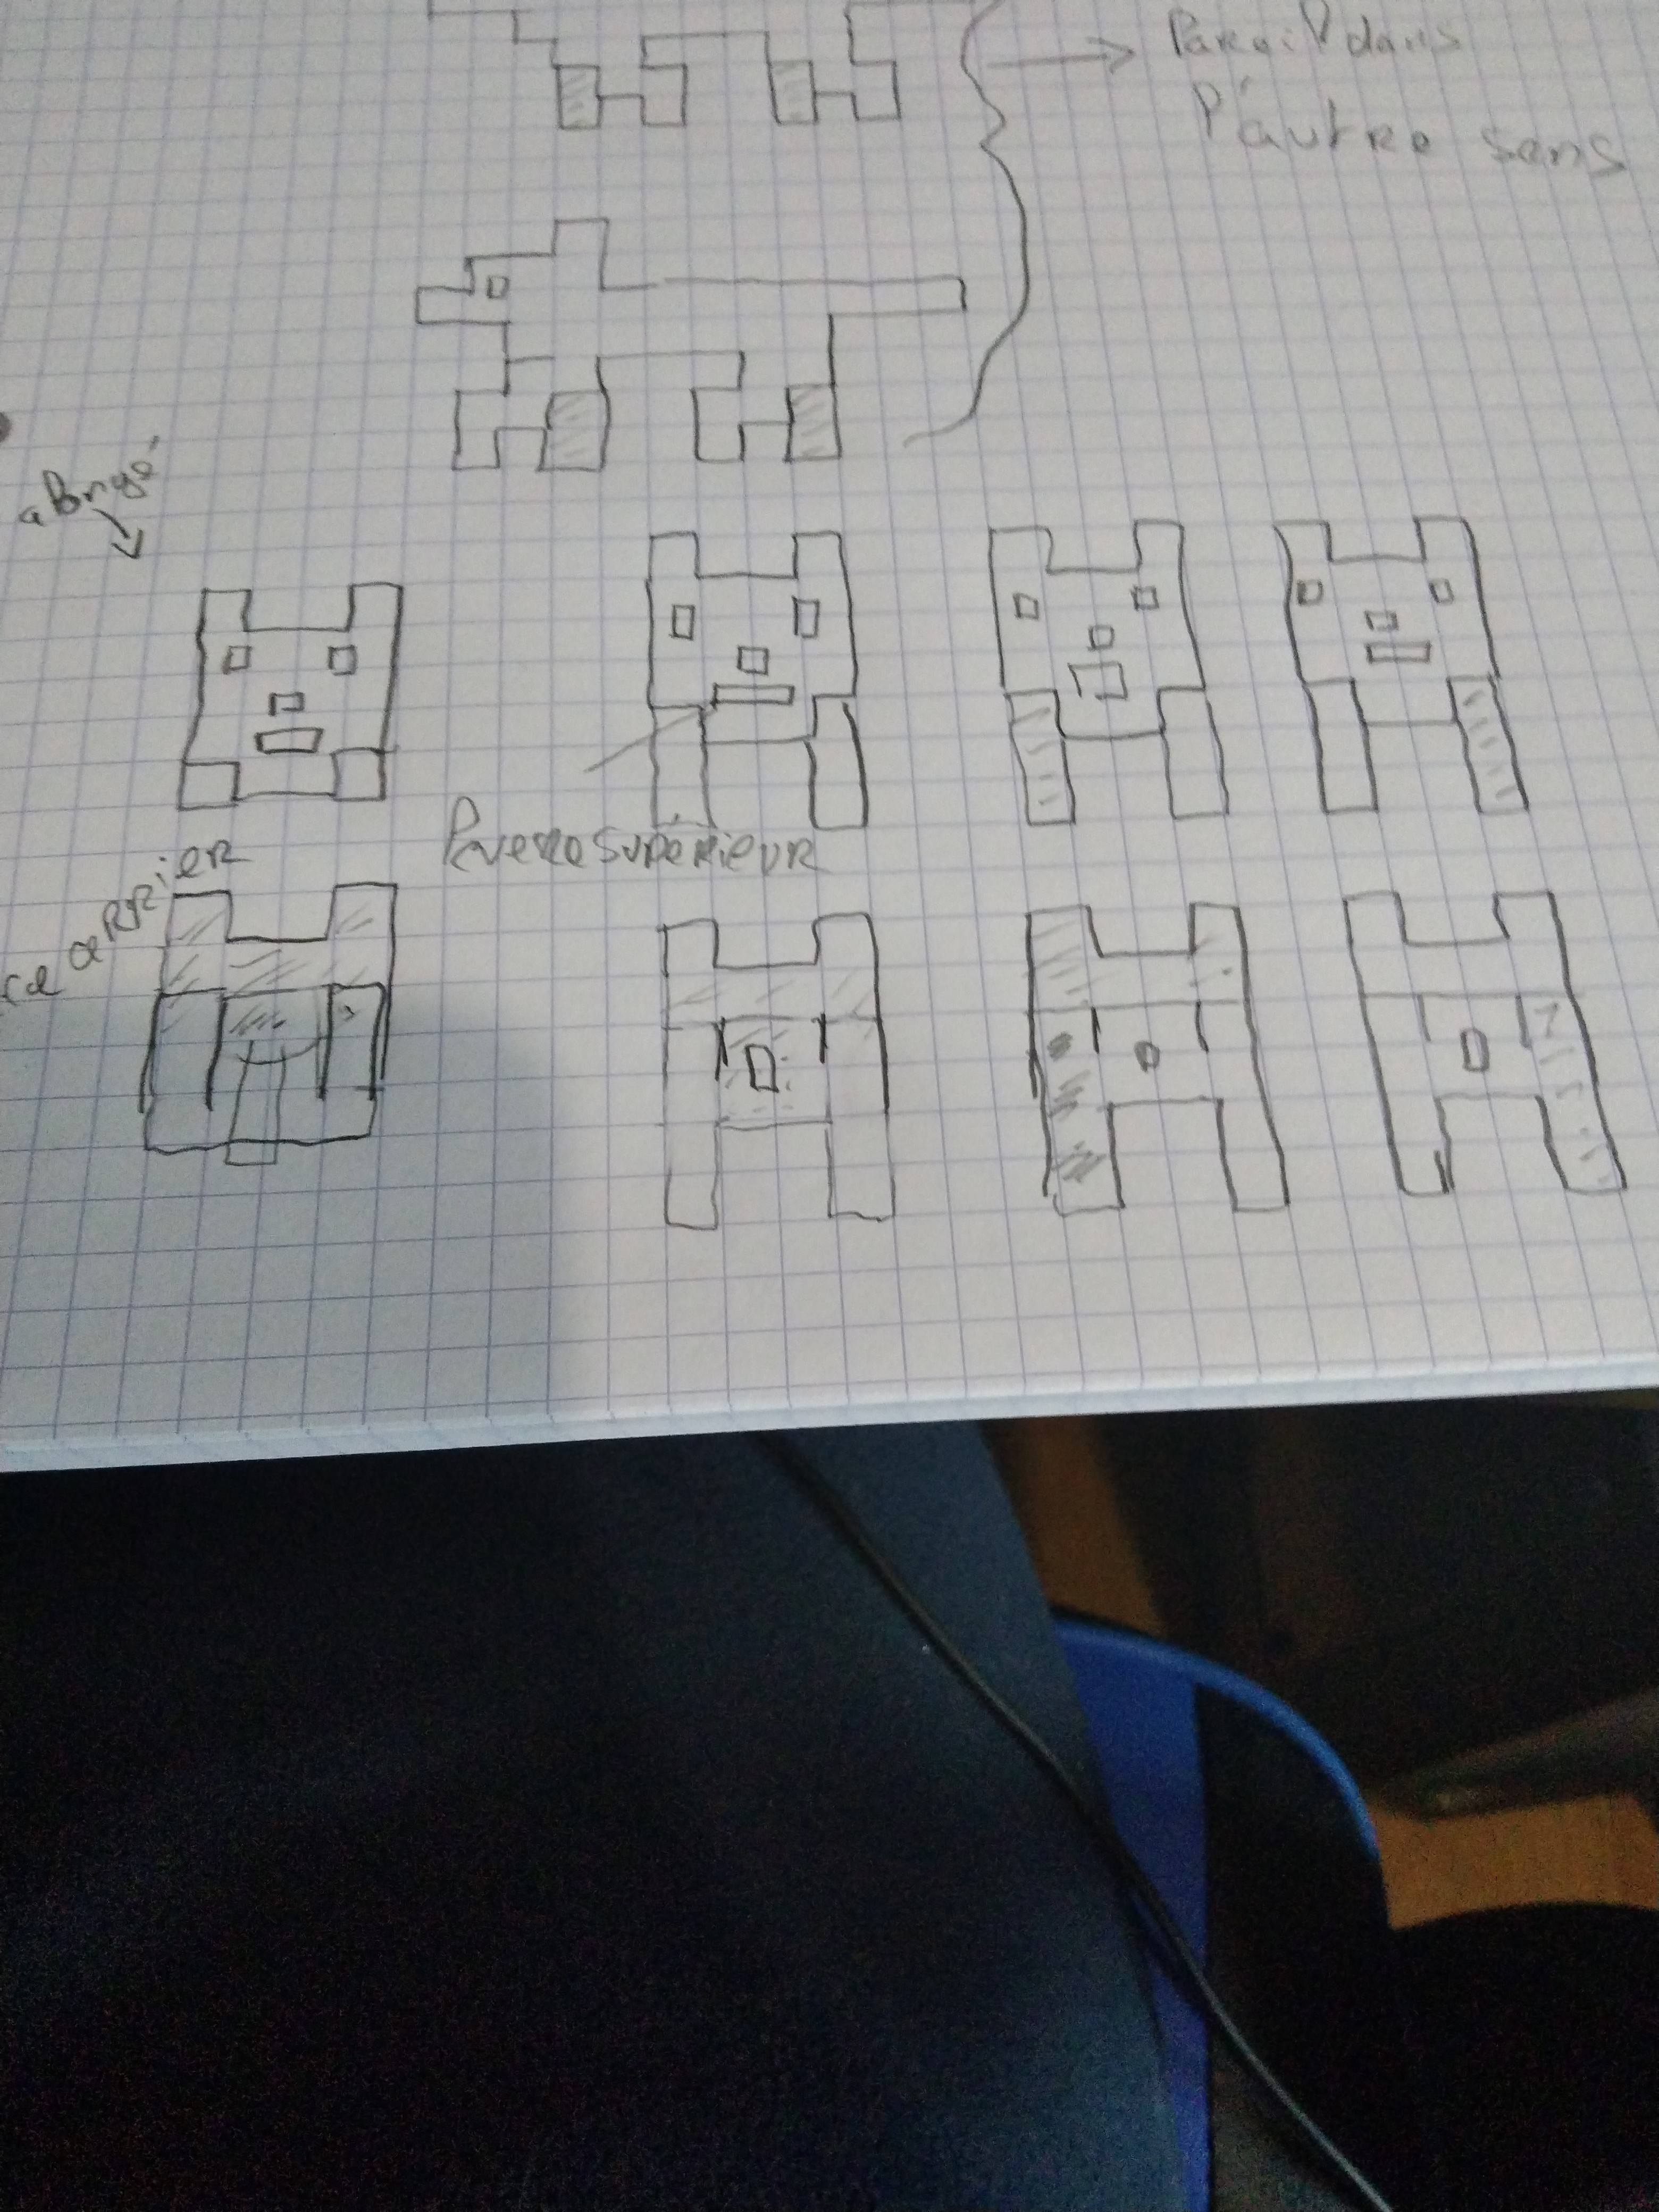
\includegraphics[width=\linewidth]{images/loup2.jpg}
  \end{minipage}
  \caption{(a) croquis du loup}
  \label{fig::example::two}
\end{figure*}
\\
\begin{figure*}[ht!]
 \centering
 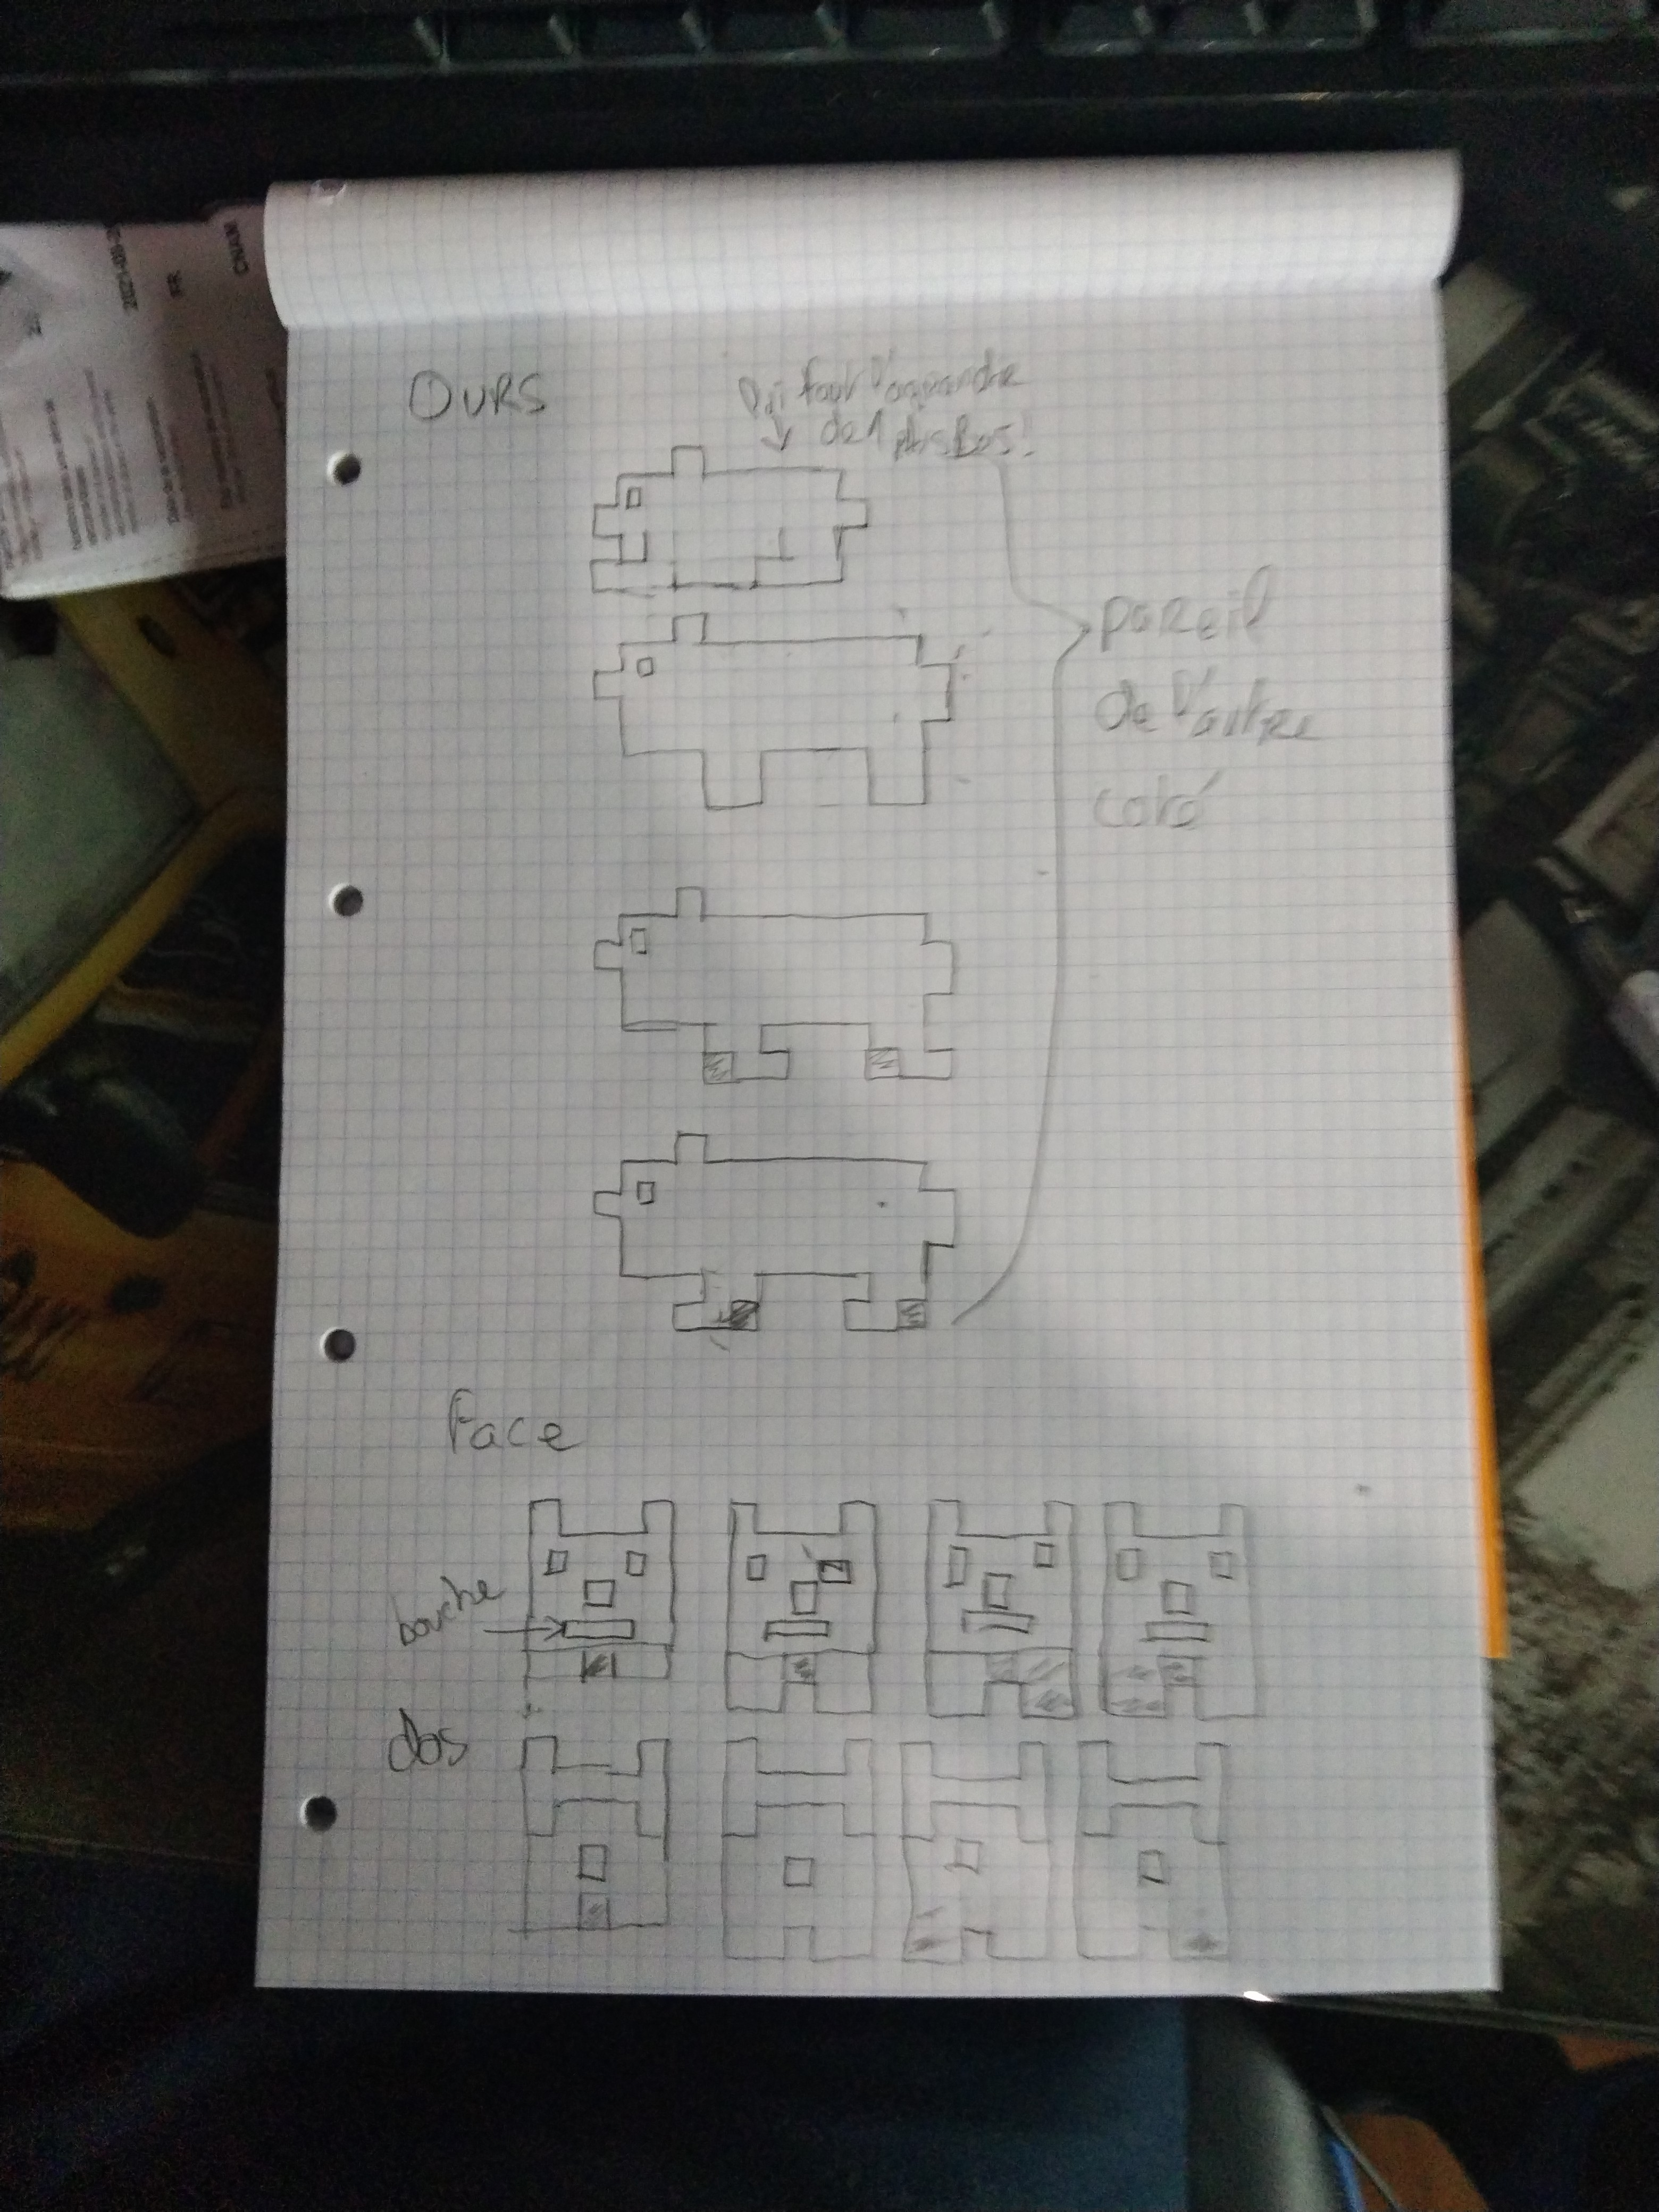
\includegraphics[width=0.5\linewidth]{images/ours.jpg}
 \caption{croquis de l'ours}
 \label{fig::example::one}
\end{figure*}
\\
\begin{figure*}[ht!]
 \centering
 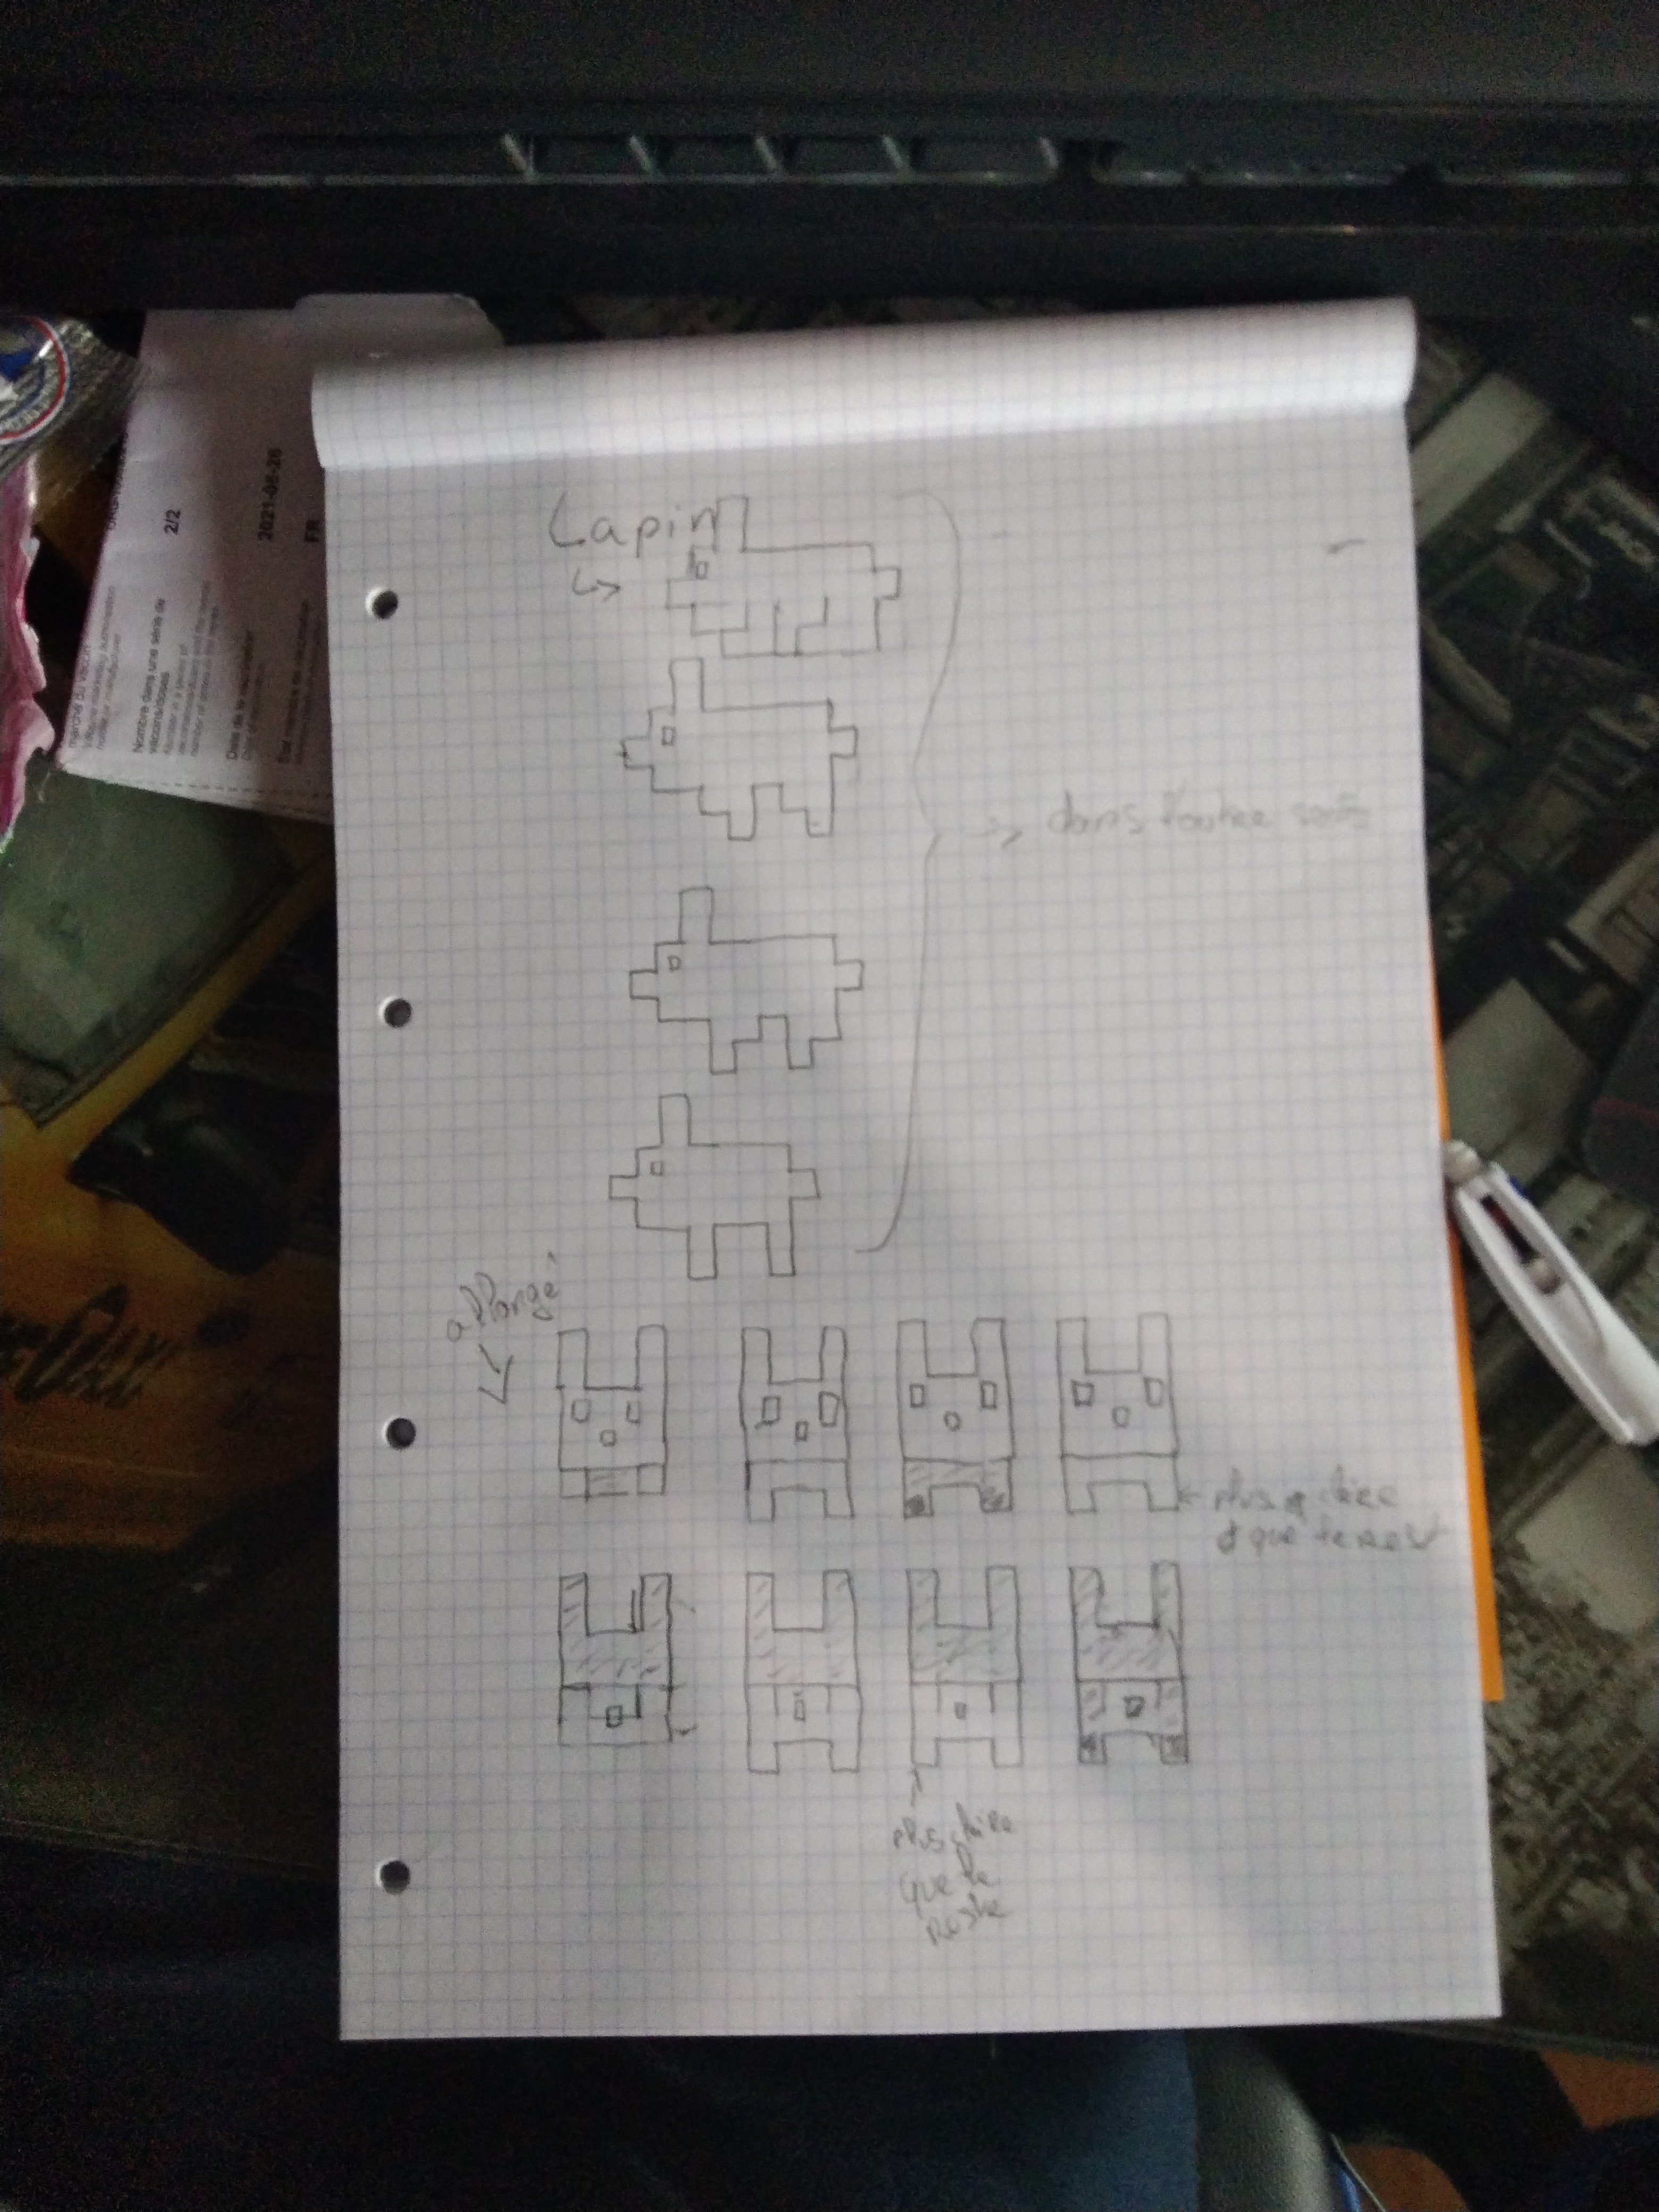
\includegraphics[width=0.5\linewidth]{images/lapin.jpg}
 \caption{croquis du lapin}
 \label{fig::example::one}
\end{figure*}
\\
\begin{figure*}[ht!]
 \centering
 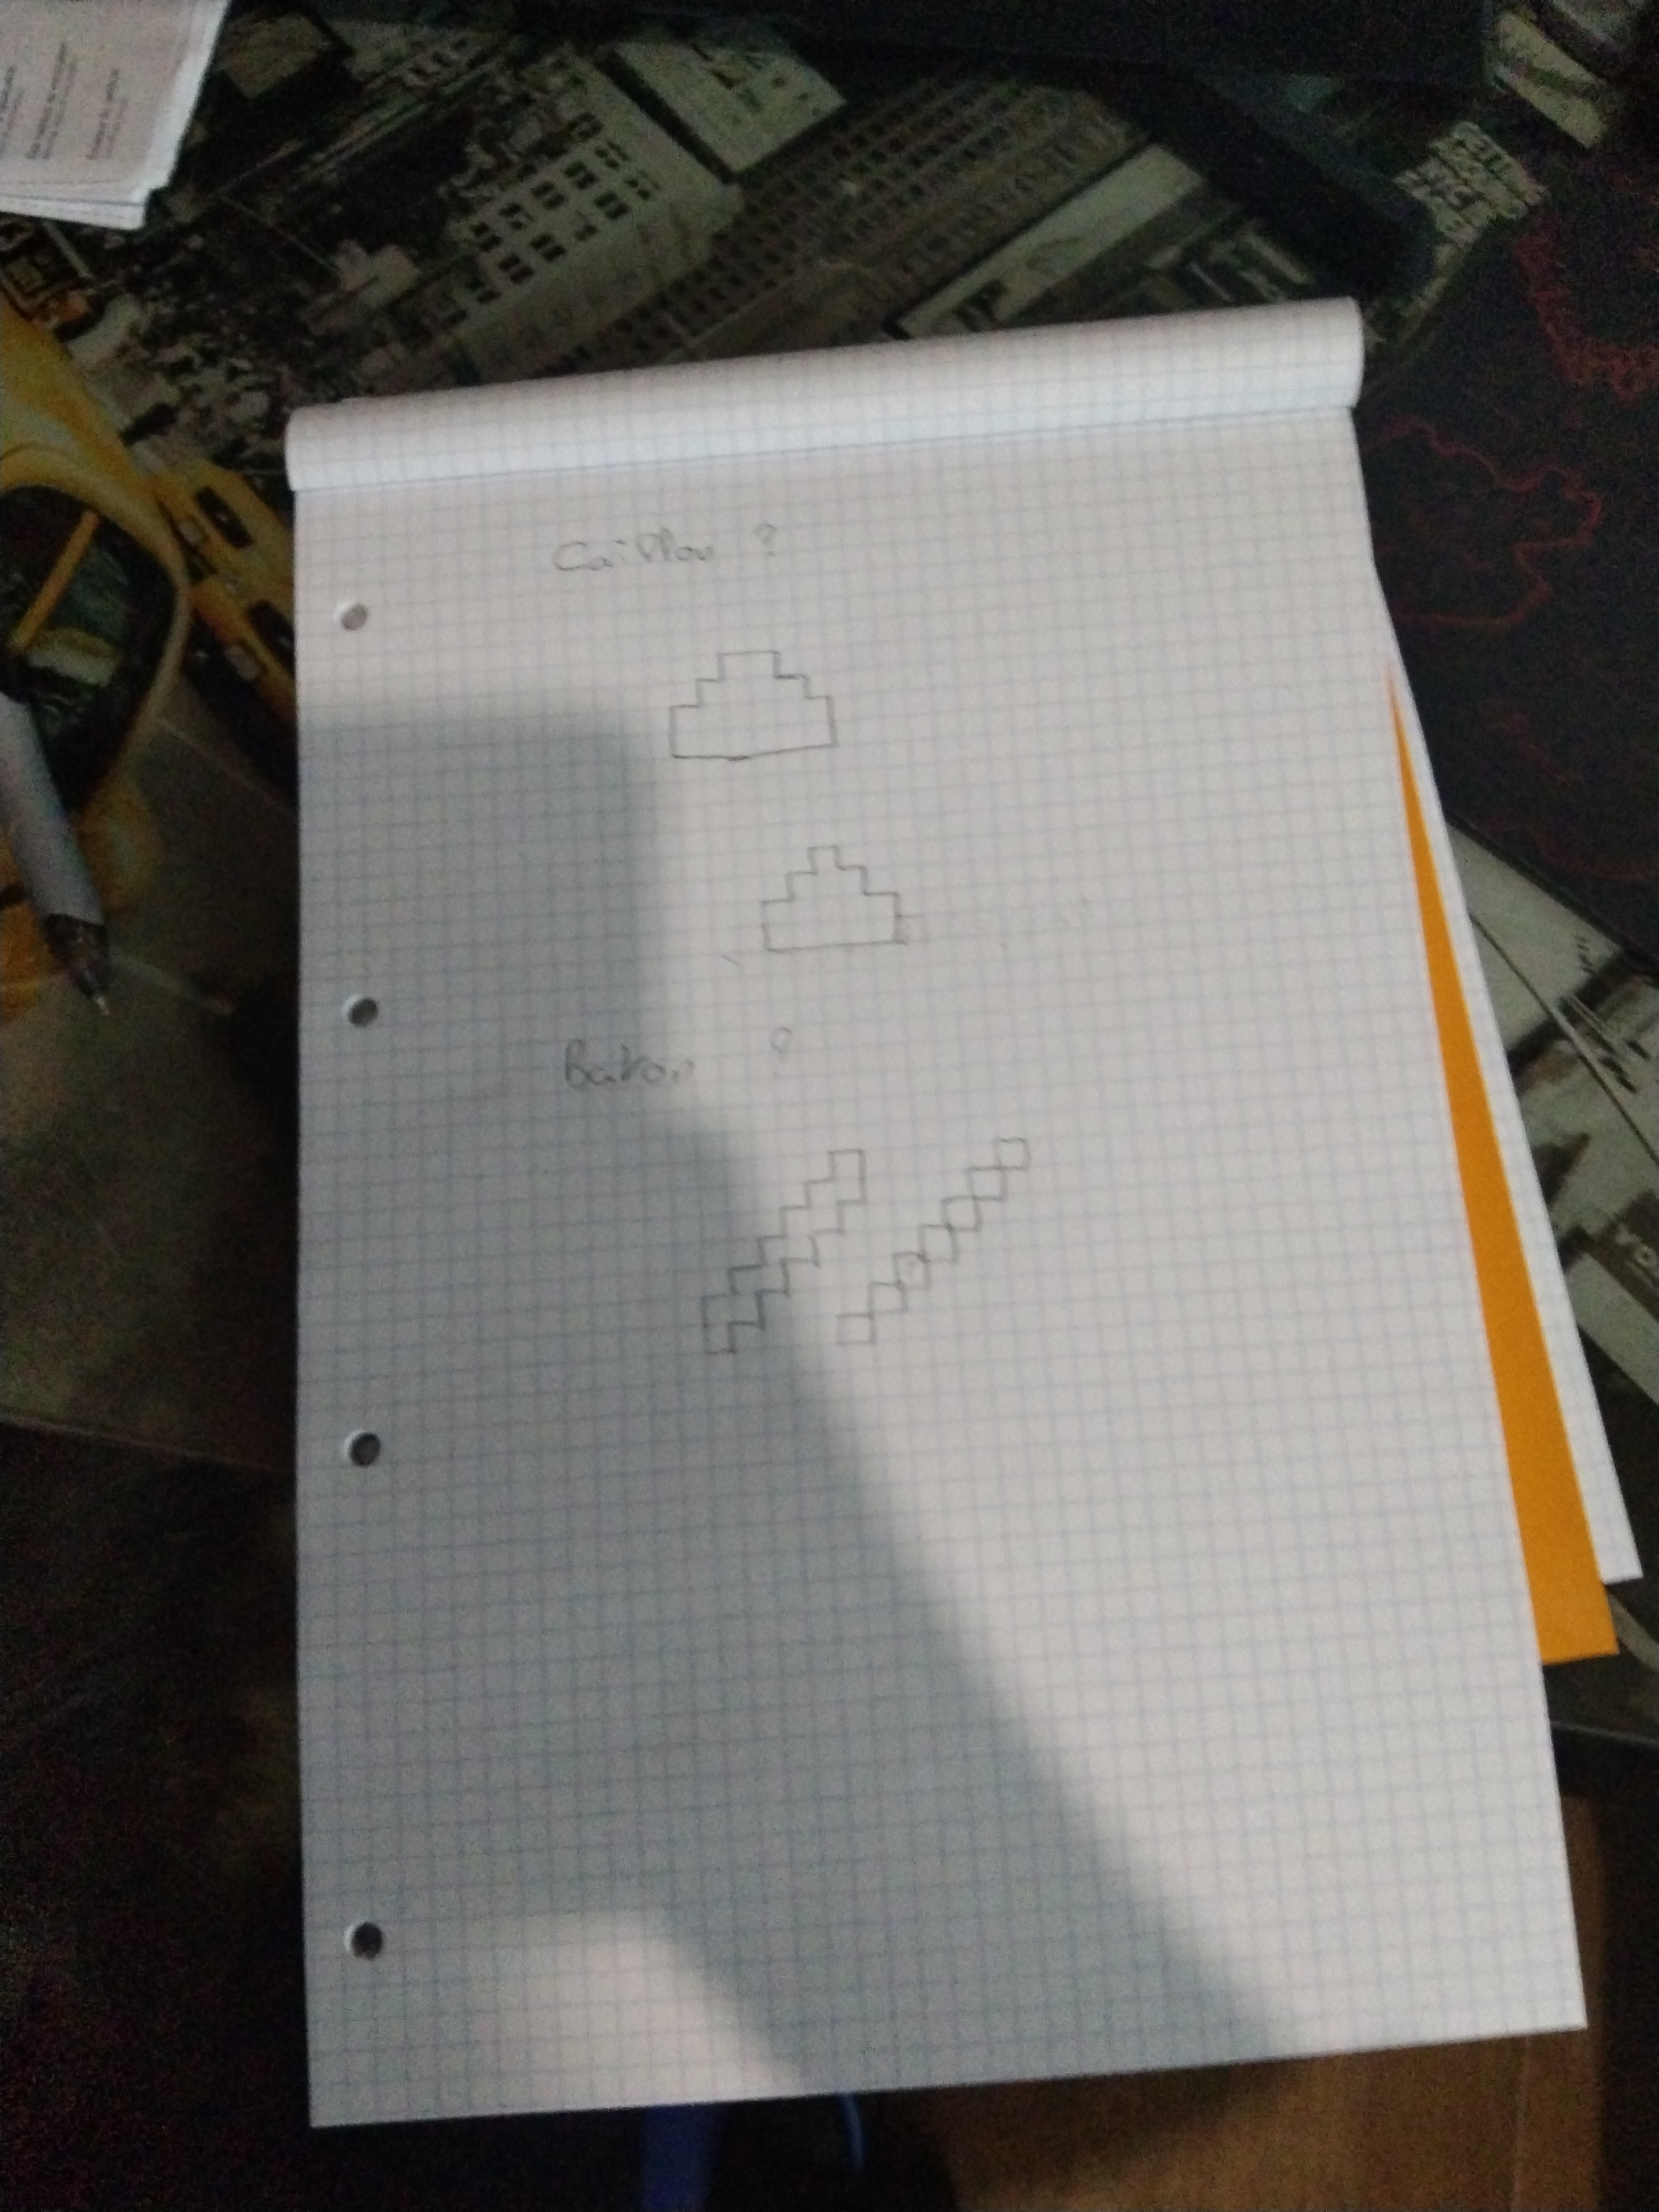
\includegraphics[width=0.5\linewidth]{images/caillou&batton}
 \caption{croquis du caillou et du bâton}
 \label{fig::example::one}
\end{figure*}
\\
\newpage
{\color{white}Ceci sert a la mise en page}
\newpage
\item Et ensuite il a donc fait les sprites de chaque entités en croquis :
\\
\begin{figure*}[ht!]
 \centering
 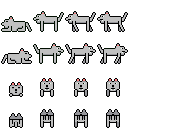
\includegraphics[width=0.5\linewidth]{images/loup.png}
 \caption{sprite du loup}
 \label{fig::example::one}
\end{figure*}
\\
\begin{figure*}[ht!]
 \centering
 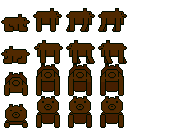
\includegraphics[width=0.5\linewidth]{images/ours.png}
 \caption{sprite de l'ours}
 \label{fig::example::one}
\end{figure*}
\\
\begin{figure*}[ht!]
  \begin{minipage}[c]{.5\linewidth}
   \centering
   
\includegraphics[width=\linewidth]{images/caillou.png}
  \end{minipage} \hfill
  \begin{minipage}[c]{.5\linewidth}
   \centering
   
\includegraphics[width=\linewidth]{images/baton.png}
  \end{minipage}
  \caption{(a) sprite du caillou ; (b) sprite du bâton}
  \label{fig::example::two}
\end{figure*}
\newpage
\item Il était sur une moyenne de 5-6 heures par sprites par jour, mais il a réparti cela sur plusieurs semaines environ 3-4.\\
\\
\item Ensuite durant un peu plus d'un mois il a fait la fenêtre de menu du jeu sur une moyenne de 4 heures par semaines.\\
\\
\item a passer même pas  minutes a faire le sprite de l'herbe :\\
\begin{figure*}[ht!]
 \centering
 
\includegraphics[width=0.3\linewidth]{images/herbe.png}
 \caption{sprite de l'herbe}
 \label{fig::example::one}
\end{figure*}
\\
\item Et enfin il a commencé le Latex le "28 mars 2022" et je l'ai fini le "23 avril 2022 ".\\
\end{enumerate}
\newpage

\section{Illustration sur un exemple concret}
les illustrations de l'exemple :\\
\begin{figure*}[ht!]
  \begin{minipage}[c]{.5\linewidth}
   \centering
   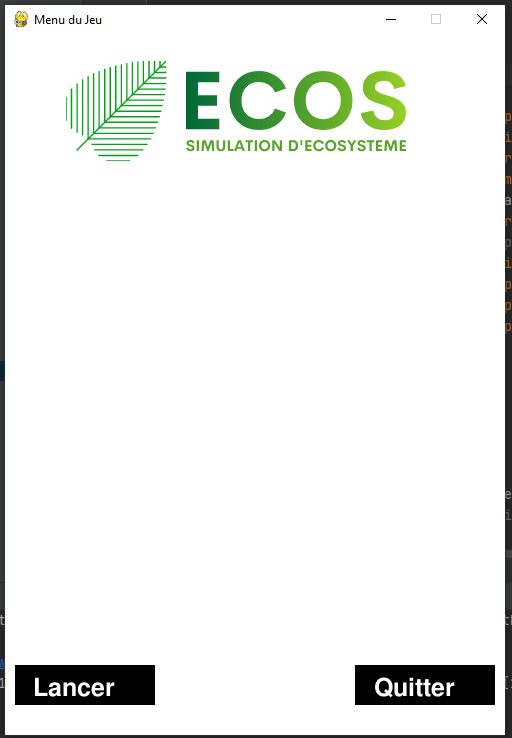
\includegraphics[width=0.75\linewidth]{images/exemple1.png}
  \end{minipage} \hfill
  \begin{minipage}[c]{.5\linewidth}
   \centering
   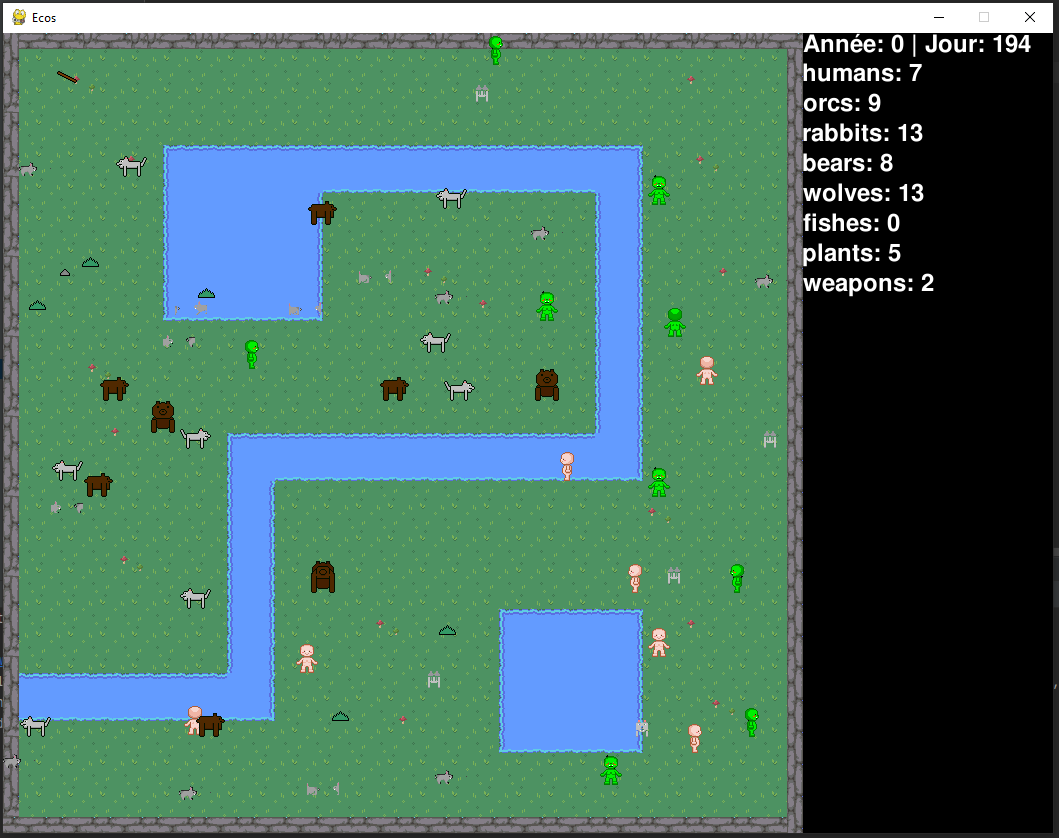
\includegraphics[width=1.5\linewidth]{images/exemple2.png}
  \end{minipage}
  \caption{(a) arriver sur le menu du jeu ; (b) arriver sur la simulation}
  \label{fig::example::two}
\end{figure*}
\newpage

\section{Les éventuels sources}

Pour les sprites : \\
		 Sprite de l'humain :
\begin{figure*}[ht!]
 \centering
 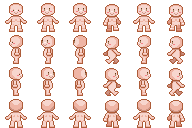
\includegraphics[width=0.5\linewidth]{images/human.png}
 \caption{Nous n'avons pas trouver de sources}
 \label{fig::example::one}
\end{figure*}
\\
		 Sprite de l'orc :
\begin{figure*}[ht!]
 \centering
 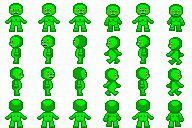
\includegraphics[width=0.5\linewidth]{images/orc.png}
 \caption{C'est une recoloration du sprite de l'humain}
 \label{fig::example::one}
\end{figure*}
\\
		 Les autres sprites : Nous n'avons pas de sources puisqu'ils ont étaient fait par nos soins.\\
Pour la texture de la map : https://stealthix.itch.io/rpg-nature-tileset  - \href{https://stealthix.itch.io/rpg-nature-tileset}{Tileset Map}\\
Pour "l'algorithme" : https://khayyam.developpez.com/articles/algo/astar/ - \href{https://khayyam.developpez.com/articles/algo/astar/}{La documentation}\\
Pour le code : fait nous même (avec aide du prof a des moment)\\

\newpage

\section{Conclusion}

Pour conclure nous aurions aimer / voulu :\\
Si nous aurions eu plus de temps nous aurions voulu faire un écran de fin, des fins alternatives, un menu pour gérer le nombre d'entité et autres.\\
\vspace{1cm}
\\
\vspace{1cm}
Merci d'avoir lu notre rapport.\\
Nous voulions remercier:\\
\begin{itemize}
\item Mr CHAHIR notre enseignant de travaux pratiques en conception logiciel, qui nous a aidez a résoudre pas mal de problème sur notre simulation d'écosystème.
\end{itemize}

\vspace{1cm}

Etudiants en L1 informatique groupe 5:\\
\begin{itemize}
\item BONVARLET Bastien\\
\item MASSON Joris\\
\item CHAMPENOIS Brandon\\
\end{itemize}

\newpage
\end{document}